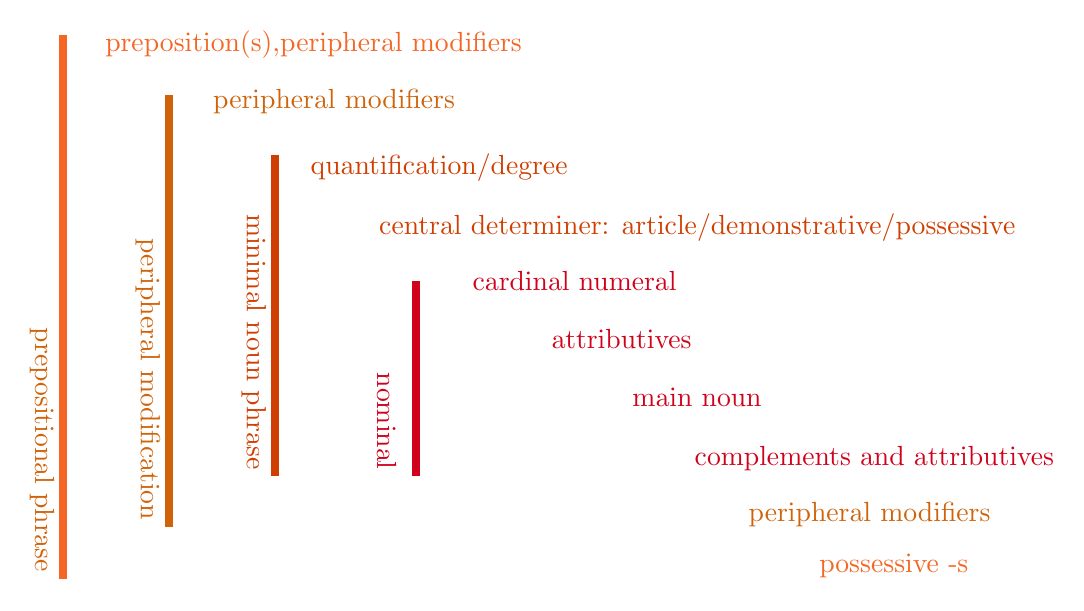
\begin{tikzpicture}[x=0.75pt,y=0.75pt,yscale=-1,xscale=1]
    %uncomment if require: \path (0,427); %set diagram left start at 0, and has height of 427
    
    %Straight Lines [id:da03551150377502288] 
    \draw [color={rgb, 255:red, 208; green, 2; blue, 27 }  ,draw opacity=1 ][fill={rgb, 255:red, 144; green, 19; blue, 254 }  ,fill opacity=1 ][line width=3]    (393,223.93) -- (393,317.93) ;
    %Straight Lines [id:da12974027648754127] 
    \draw [color={rgb, 255:red, 208; green, 63; blue, 2 }  ,draw opacity=1 ][fill={rgb, 255:red, 74; green, 144; blue, 226 }  ,fill opacity=1 ][line width=3]    (325,162.93) -- (325,317.93) ;
    %Straight Lines [id:da790063550615397] 
    \draw [color={rgb, 255:red, 208; green, 99; blue, 10 }  ,draw opacity=1 ][fill={rgb, 255:red, 74; green, 144; blue, 226 }  ,fill opacity=1 ][line width=3]    (274,134.26) -- (274,342.26) ;
    %Straight Lines [id:da5340823111898327] 
    \draw [color={rgb, 255:red, 245; green, 101; blue, 35 }  ,draw opacity=1 ][fill={rgb, 255:red, 74; green, 144; blue, 226 }  ,fill opacity=1 ][line width=3]    (223,105.26) -- (223,367.26) ;
    
    % Text Node
    \draw (374,190) node [anchor=north west][inner sep=0.75pt]  [color={rgb, 255:red, 208; green, 63; blue, 2 }  ,opacity=1 ] [align=left] {central determiner: article/demonstrative/possessive};
    % Text Node
    \draw (419,218) node [anchor=north west][inner sep=0.75pt]  [color={rgb, 255:red, 208; green, 2; blue, 27 }  ,opacity=1 ] [align=left] {cardinal numeral};
    % Text Node
    \draw (457,246) node [anchor=north west][inner sep=0.75pt]  [color={rgb, 255:red, 208; green, 2; blue, 27 }  ,opacity=1 ] [align=left] {attributives};
    % Text Node
    \draw (496,274) node [anchor=north west][inner sep=0.75pt]  [color={rgb, 255:red, 208; green, 2; blue, 27 }  ,opacity=1 ] [align=left] {main noun};
    % Text Node
    \draw (341,161) node [anchor=north west][inner sep=0.75pt]  [color={rgb, 255:red, 208; green, 63; blue, 2 }  ,opacity=1 ] [align=left] {quantification/degree};
    % Text Node
    \draw (526,302) node [anchor=north west][inner sep=0.75pt]  [color={rgb, 255:red, 208; green, 2; blue, 27 }  ,opacity=1 ] [align=left] {complements and attributives};
    % Text Node
    \draw (373,315.93) node [anchor=south east] [inner sep=0.75pt]  [color={rgb, 255:red, 208; green, 2; blue, 27 }  ,opacity=1 ,rotate=-90] [align=left] {nominal};
    % Text Node
    \draw (322,315.93) node [anchor=north east] [inner sep=0.75pt]  [color={rgb, 255:red, 208; green, 63; blue, 2 }  ,opacity=1 ,rotate=-90] [align=left] {minimal noun phrase};
    % Text Node
    \draw (271,340.26) node [anchor=north east] [inner sep=0.75pt]  [color={rgb, 255:red, 208; green, 99; blue, 10 }  ,opacity=1 ,rotate=-90] [align=left] {peripheral modification};
    % Text Node
    \draw (294,130) node [anchor=north west][inner sep=0.75pt]  [color={rgb, 255:red, 208; green, 99; blue, 10 }  ,opacity=1 ] [align=left] {peripheral modifiers};
    % Text Node
    \draw (242,102) node [anchor=north west][inner sep=0.75pt]  [color={rgb, 255:red, 245; green, 101; blue, 35 }  ,opacity=1 ] [align=left] {preposition(s),peripheral modifiers};
    % Text Node
    \draw (220,365.26) node [anchor=north east] [inner sep=0.75pt]  [color={rgb, 255:red, 208; green, 99; blue, 10 }  ,opacity=1 ,rotate=-90] [align=left] {prepositional phrase};
    % Text Node
    \draw (552,329) node [anchor=north west][inner sep=0.75pt]  [color={rgb, 255:red, 208; green, 99; blue, 10 }  ,opacity=1 ] [align=left] {peripheral modifiers};
    % Text Node
    \draw (586,354) node [anchor=north west][inner sep=0.75pt]  [color={rgb, 255:red, 245; green, 101; blue, 35 }  ,opacity=1 ] [align=left] {possessive -s};
    
    
    \end{tikzpicture}
    